\documentclass{article}
\usepackage[margin=2cm]{geometry}
\usepackage[latin1]{inputenc}
\usepackage{todo}
\usepackage{url}
\usepackage{caption}
\usepackage{subcaption}
\usepackage{graphicx}
\usepackage{listings}
\usepackage{color}
\usepackage{textcomp}
\usepackage{float}

\definecolor{gainsboro}{rgb}{0.86, 0.86, 0.86}

\lstset{frame=tb,
  aboveskip=3mm,
  belowskip=3mm,
  showstringspaces=false,
  columns=flexible,
  basicstyle={\small\ttfamily},
  numbers=none,
  breaklines=true,
  breakatwhitespace=true,
  tabsize=4,
  language=C
}

\title{The World of Quantum Mechanics}
\author{Knut Andre G. Prestsveen}
\begin{document}
\maketitle


\section{Abstract}

\section{Introduction}

\section{Theory and method}

\section{Results}

\section{Conclusion}

\section{TEMPORARY FIG STORAGE}

\begin{figure}
    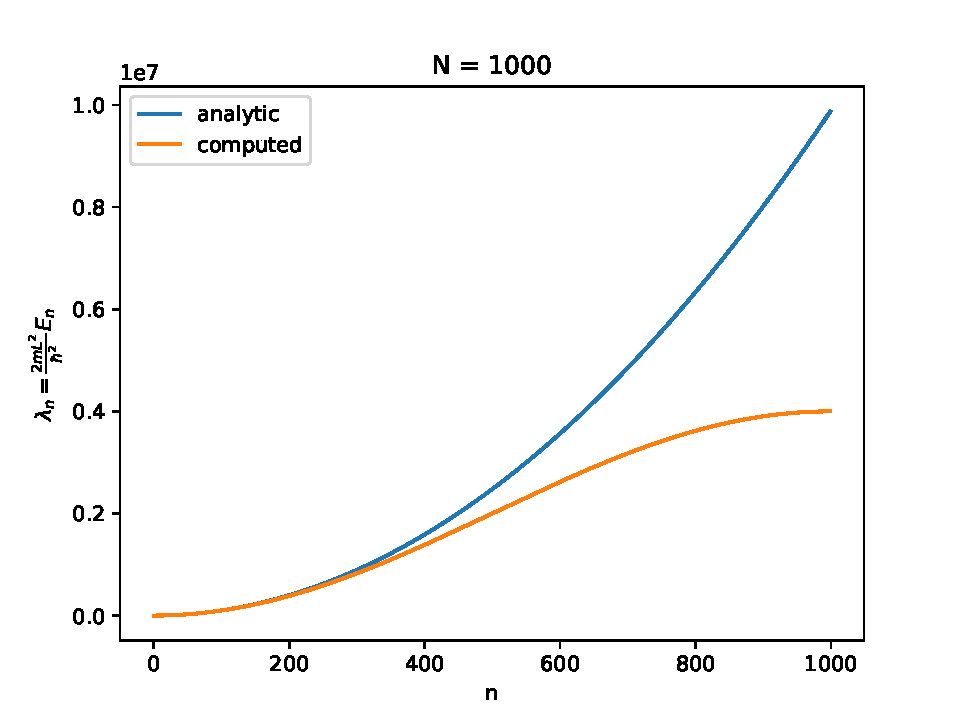
\includegraphics[width=\linewidth]{./media/eigenvalues_empty_box.pdf}
    \caption{Empty box ev}
    \label{fig:box-eigenvals}
\end{figure}

\begin{figure}
    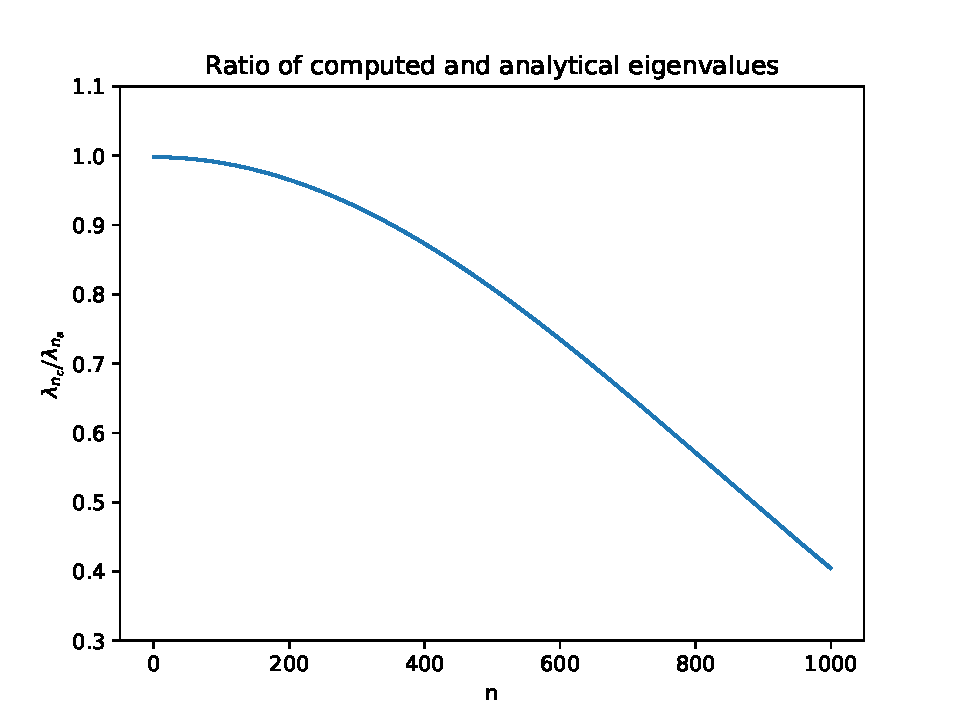
\includegraphics[width=\linewidth]{./media/eigenval_ratio_empty_box.pdf}
    \caption{Empty box ev ratio}
    \label{fig:box-eigenvals-ratio}
\end{figure}

\begin{figure}
    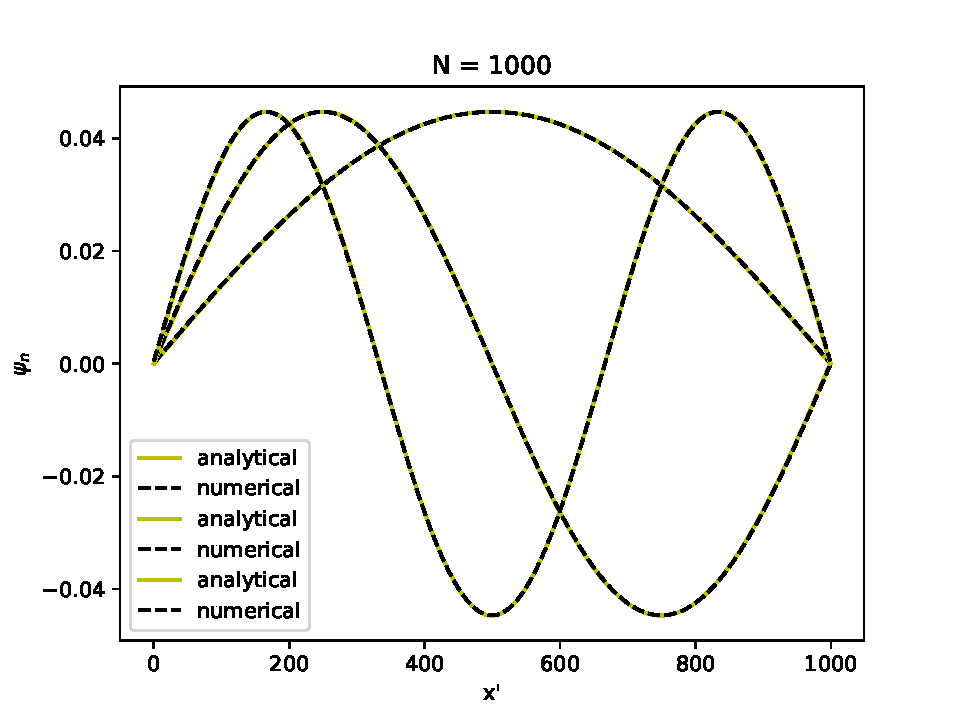
\includegraphics[width=\linewidth]{./media/eigenstates_empty_box.pdf}
    \caption{Empty box es}
    \label{fig:box-eigenstates}
\end{figure}

\begin{figure}
    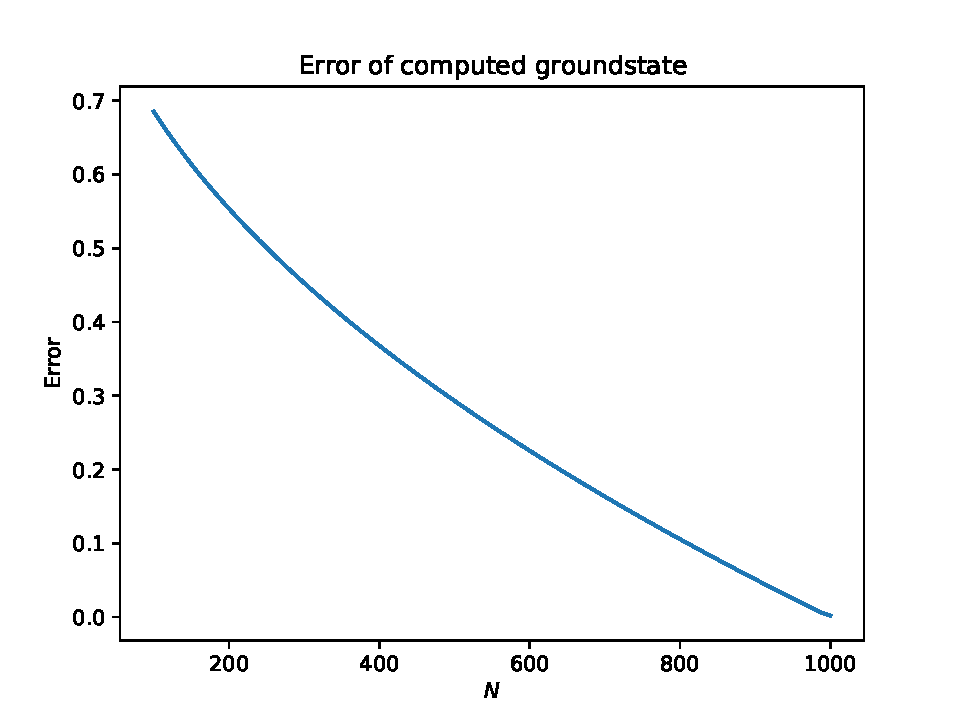
\includegraphics[width=\linewidth]{./media/wf_error_scaling.pdf}
    \caption{Empty box error scaling wf}
    \label{fig:box-eigenstates-error}
\end{figure}

\begin{figure}
    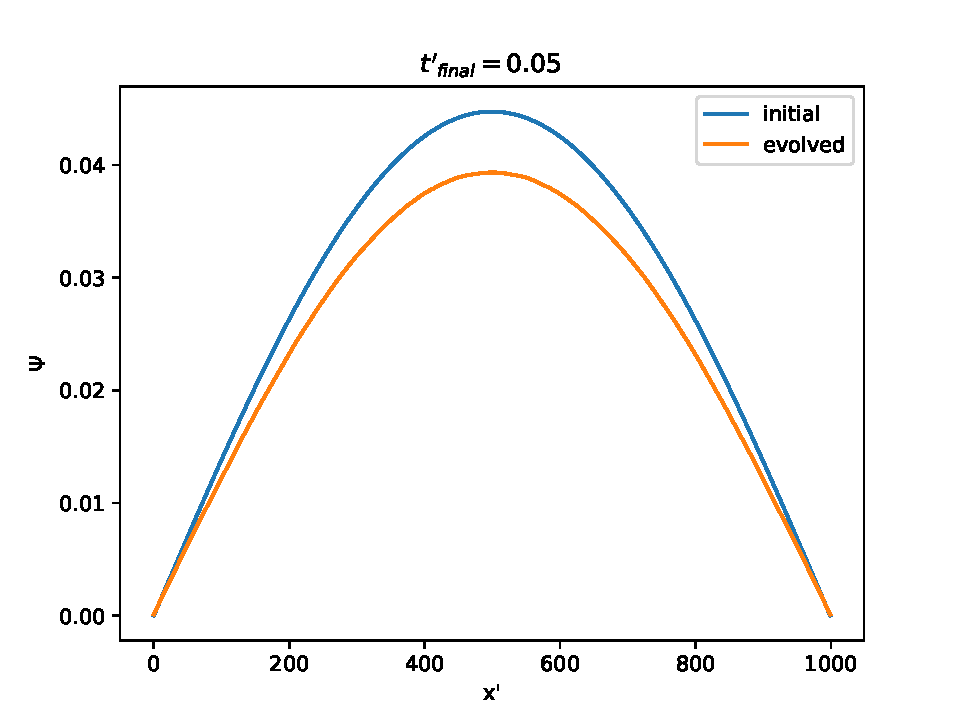
\includegraphics[width=\linewidth]{./media/time_evolve_emptybox_1.pdf}
    \caption{Empty box, time evolved1}
    \label{fig:box-time-evolved1}
\end{figure}

\begin{figure}
    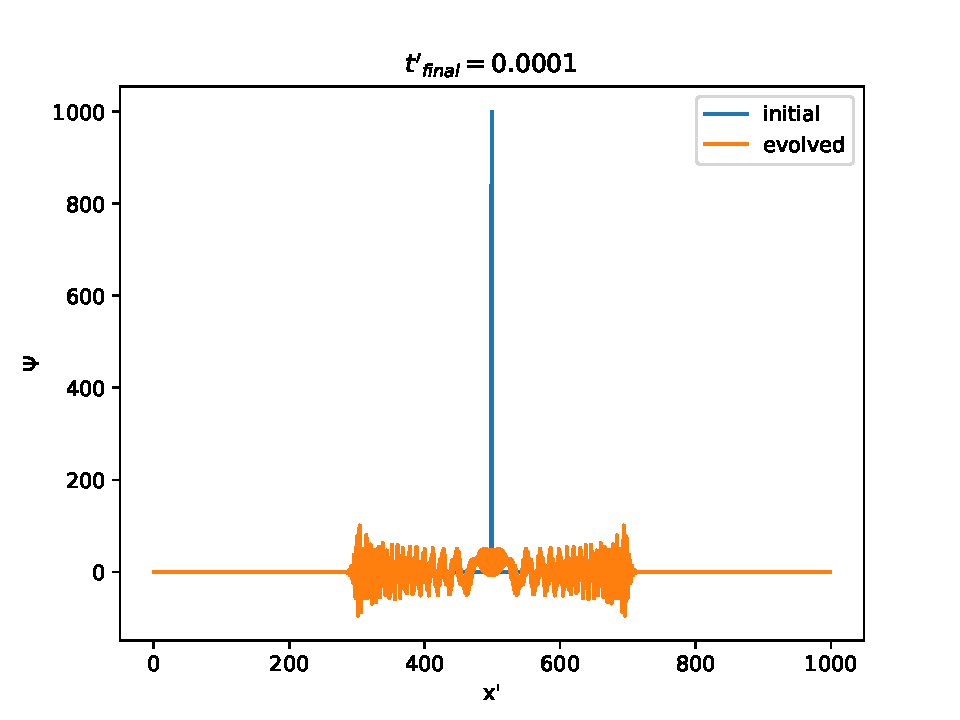
\includegraphics[width=\linewidth]{./media/time_evolve_emptybox_2.pdf}
    \caption{Empty box, time evolved2}
    \label{fig:box-time-evolved2}
\end{figure}

// BARRIER START

\begin{figure}
    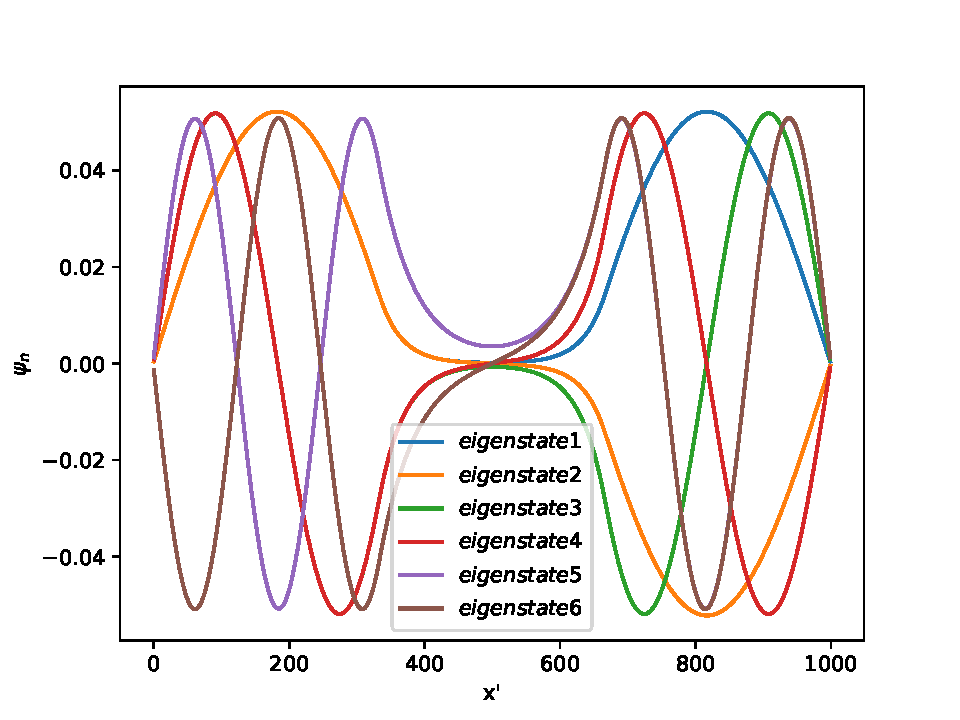
\includegraphics[width=\linewidth]{./media/bound_eigenstates_barrier.pdf}
    \caption{Barrier bound states}
    \label{fig:barrier-bound-states}
\end{figure}

\begin{figure}
    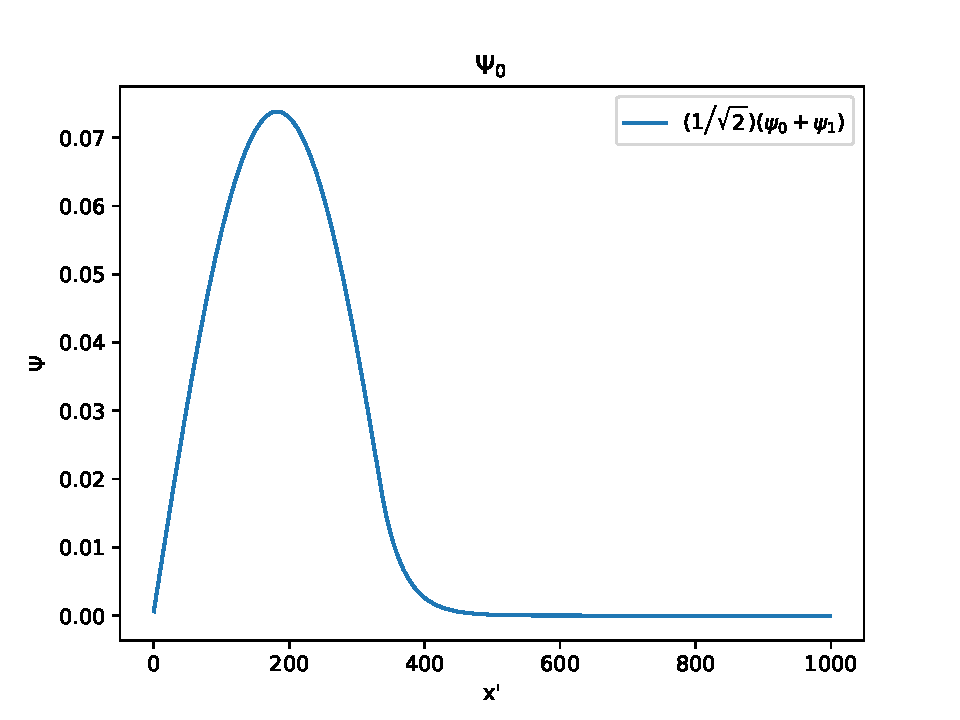
\includegraphics[width=\linewidth]{./media/initial_state.pdf}
    \caption{Barrier initial state}
    \label{fig:barrier-initial-state}
\end{figure}

\begin{figure}
    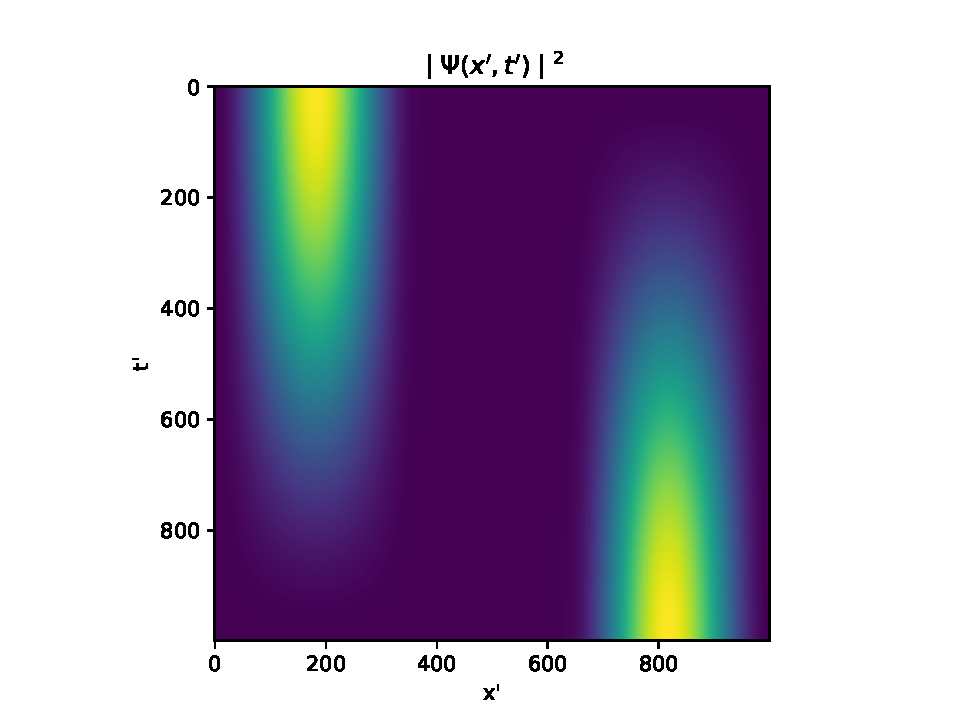
\includegraphics[width=\linewidth]{./media/time_evolve_surface.pdf}
    \caption{Barrier time evolve, surface}
    \label{fig:barrier-evolve-surface}
\end{figure}

\begin{figure}
    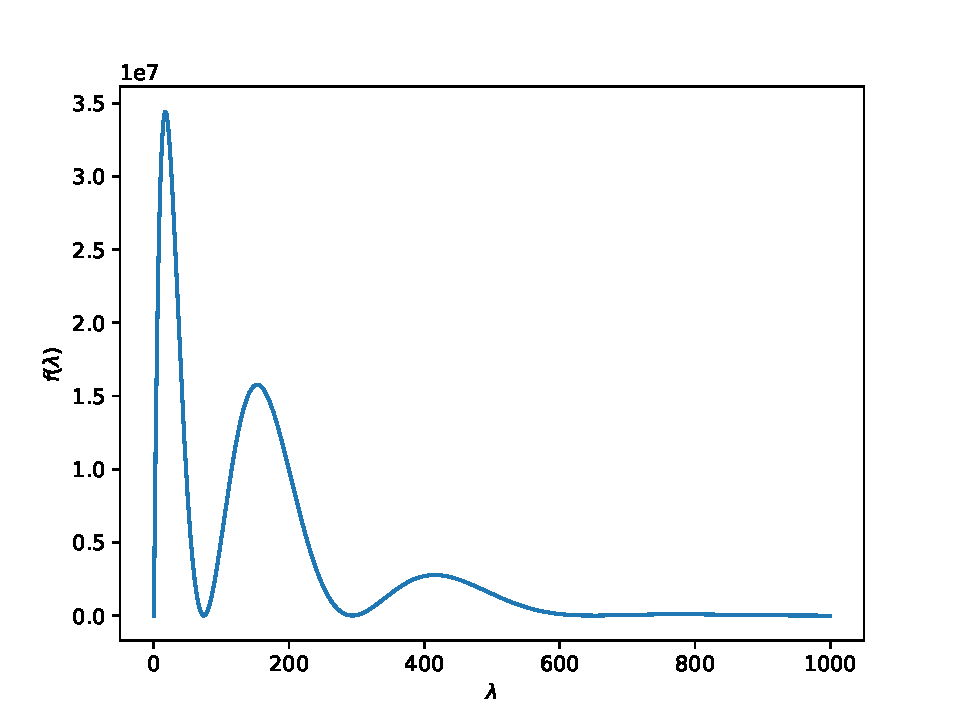
\includegraphics[width=\linewidth]{./media/f_of_lambda_roots.pdf}
    \caption{Barrier roots}
    \label{fig:barrier-roots}
\end{figure}

// TASK 3.6 TODOTODO

// STEP TIME EVOLVE START

\begin{figure}
    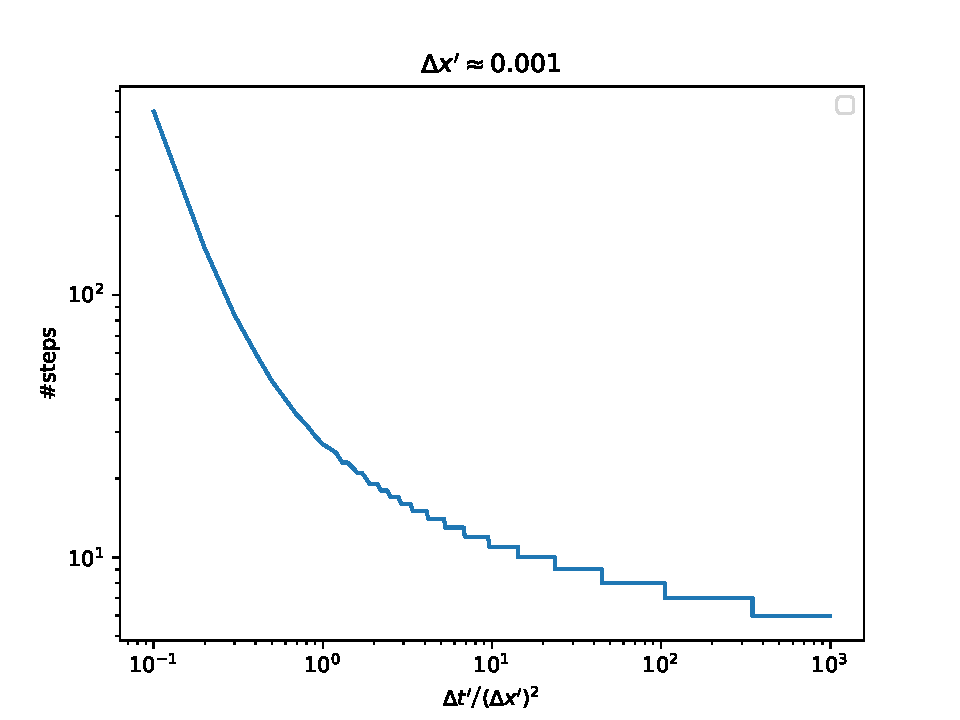
\includegraphics[width=\linewidth]{./media/steps_before_euler_collapse.pdf}
    \caption{Euler collapse}
    \label{fig:euler-collapse}
\end{figure}

\begin{figure}
    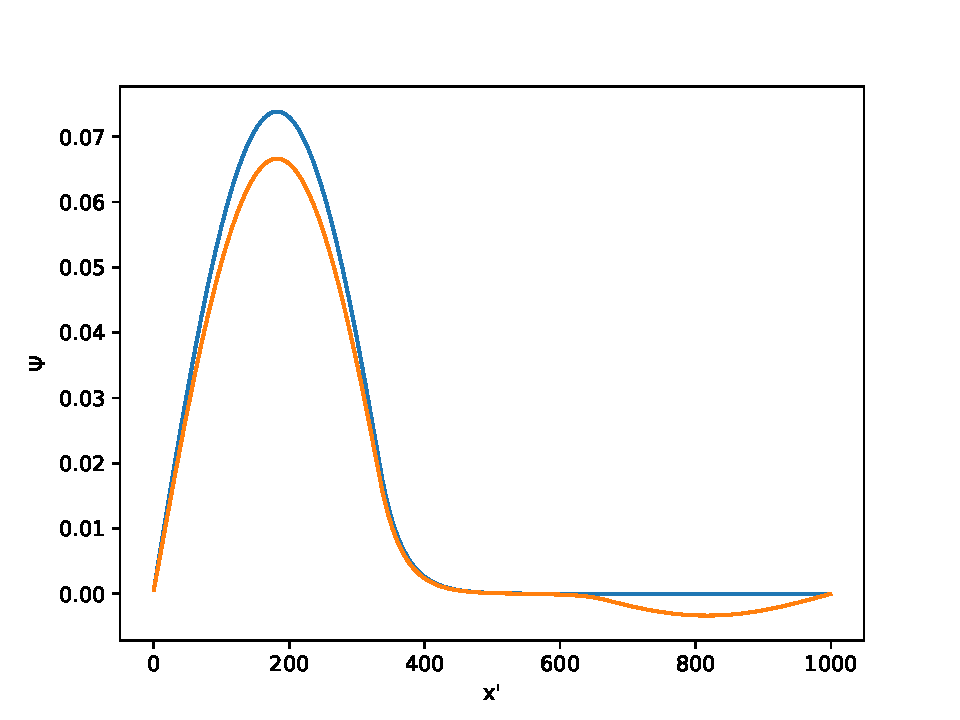
\includegraphics[width=\linewidth]{./media/crank_nicolson.pdf}
    \caption{Crank Nicolson}
    \label{fig:crank-nicolson}
\end{figure}

\end{document}






